\documentclass{beamer}
\usepackage[utf8]{inputenc}
\usetheme{Madrid}
\usecolortheme{default}
\usepackage{amsmath,amssymb,amsfonts,amsthm}
\usepackage{txfonts}
\usepackage{tk\documentclass{beamer}
\usepackage[utf8]{inputenc}

\usetheme{Madrid}
\usecolortheme{default}
\usepackage{amsmath,amssymb,amsfonts,amsthm}
\usepackage{txfonts}
\usepackage{tkz-euclide}
\usepackage{listings}
\usepackage{adjustbox}
\usepackage{array}
\usepackage{tabularx}
\usepackage{gvv}
\usepackage{lmodern}
\usepackage{circuitikz}
\usepackage{tikz}
\usepackage{graphicx}

\setbeamertemplate{page number in head/foot}[totalframenumber]

\usepackage{tcolorbox}
\tcbuselibrary{minted,breakable,xparse,skins}



\definecolor{bg}{gray}{0.95}
\DeclareTCBListing{mintedbox}{O{}m!O{}}{%
	breakable=true,
	listing engine=minted,
	listing only,
	minted language=#2,
	minted style=default,
	minted options={%
		linenos,
		gobble=0,
		breaklines=true,
		breakafter=,,
		fontsize=\small,
		numbersep=8pt,
		#1},
	boxsep=0pt,
	left skip=0pt,
	right skip=0pt,
	left=25pt,
	right=0pt,
	top=3pt,
	bottom=3pt,
	arc=5pt,
	leftrule=0pt,
	rightrule=0pt,
	bottomrule=2pt,
	toprule=2pt,
	colback=bg,
	colframe=orange!70,
	enhanced,
	overlay={%
		\begin{tcbclipinterior}
			\fill[orange!20!white] (frame.south west) rectangle ([xshift=20pt]frame.north west);
	\end{tcbclipinterior}},
	#3,
}
\lstset{
	language=C,
	basicstyle=\ttfamily\small,
	keywordstyle=\color{blue},
	stringstyle=\color{orange},
	commentstyle=\color{green!60!black},
	numbers=left,
	numberstyle=\tiny\color{gray},
	breaklines=true,
	showstringspaces=false,
}
%------------------------------------------------------------
%This block of code defines the information to appear in the
%Title page
\title %optional
{5.2.49}
%\subtitle{A short story}

\author % (optional)
{RAVULA SHASHANK REDDY - EE25BTECH11047}

 \begin{document}
	
	
	\frame{\titlepage}
	\begin{frame}{Question}
    Find the parameters of the conic
\begin{align*}
   36x^2+4y^2=144. 
\end{align*}

\end{frame}
\begin{frame}{Solution}
    \begin{align}
g(\vec{x}) &= \vec{x}^\top \vec{V} \vec{x} + 2\vec{u}^\top \vec{x} + f = 0 \\
\vec{V} &= \myvec{36 & 0 \\ 0 & 4}, \quad 
\vec{u}=\myvec{0\\0}, \quad 
f=-144\\
\lambda_1 &= 36, \quad \lambda_2 = 4 \\
\end{align}
Since $\lambda_1 > \lambda_2$, apply affine transformation
\begin{align}
\vec{P} &= \myvec{0 & 1 \\ 1 & 0}, \quad \vec{x} = \vec{P}\vec{y}
\end{align}

Hence,
\begin{align}
\lambda_1 &= 4, \quad \lambda_2 = 36 \\
\vec{e}_1 &= \vec{p}_2 = \myvec{0\\1}, \quad
\vec{e}_2 = \vec{p}_1 = \myvec{1\\0}
\end{align}
\end{frame}
\begin{frame}{Solution}
\begin{align}
f_0 &= \vec{u}^\top \vec{V}^{-1}\vec{u} - f = 144\\
e &= \sqrt{1-\frac{\lambda_1}{\lambda_2}}
= \sqrt{1-\frac{4}{36}}
= \frac{2\sqrt{2}}{3}\\
\text{Major axis} &= 2\sqrt{\frac{f_0}{\lambda_1}}
= 12 \\
\text{Minor axis} &= 2\sqrt{\frac{f_0}{\lambda_2}}
= 4
\end{align}
Normal vector of directrix:
\begin{align}
\vec{n} &= \sqrt{\lambda_2}\,\vec{p}_2 
= \sqrt{36}\myvec{0\\1} 
= \myvec{0\\6}\\
\vec{p}_1 &= \myvec{1\\0}, \quad \vec{p}_2 = \myvec{0\\1}
\end{align}
\end{frame}
\begin{frame}{Solution}
\begin{align}
c &= \frac{e\,\vec{u}^\top\vec{n} \;\pm\; 
\sqrt{\,e^{2}\left(\vec{u}^\top\vec{n}\right)^{2} 
- \lambda_{2}\left(e^{2}-1\right)\left(\|\vec{u}\|^{2}-\lambda_{2}f\right)}}{\lambda_{2}e\left(e^{2}-1\right)} \\[6pt]
c &= \pm\frac{1}{e}\sqrt{\frac{\lambda_2 f_0}{\lambda_1}}
= \pm\frac{1}{e}\sqrt{\frac{36\cdot144}{4}}
= \pm 27\sqrt{2} 
\end{align}
Foci:
\begin{align}
\vec{F} &= \frac{c e^2 \vec{n} - \vec{u}}{\lambda_2} 
= \pm 4\sqrt{2}\vec{e}_2
\end{align}
Directrices:
\begin{align}
\vec{n}^\top \vec{x} &= \pm 27\sqrt{2}\\
6\vec{e_2}^\top \vec{x} &= \pm 27\sqrt{2}\\
\vec{e_2}^\top \vec{x} &= \pm \frac{9\sqrt{2}}{2}
\end{align}
\end{frame}
\begin{frame}{Solution}
Latus rectum:
\begin{align}
l &= \frac{2\sqrt{|f_0 \lambda_1|}}{\lambda_2}
= \frac{4}{3}
\end{align}

\[
\begin{array}{|c|c|}
\hline
\text{Parameter} & \text{Value} \\
\hline
\vec{V},\;\vec{u},\;f & 
\myvec{36 & 0\\0 & 4}, \; \vec{0}, \; -144 \\
\hline
\lambda_1,\lambda_2 & 4,\;36 \\
\hline
f_0 & 144 \\
\hline
e & \tfrac{2\sqrt{2}}{3} \\
\hline
\text{Major axis length} & 12 \\
\hline
\text{Minor axis length} & 4 \\
\hline
\text{Foci} & \vec{F}=\pm 4\sqrt{2}\,\vec{e}_2 \\
\hline
\text{Directrices} & \vec{e}_2^\top \vec{x} = \pm \tfrac{9\sqrt{2}}{2} \\
\hline
\text{Latus rectum} & \tfrac{4}{3} \\
\hline
\end{array}
\]

\end{frame}
\begin{frame}[fragile]
    \frametitle{C Code}
    \begin{lstlisting}
        #include <stdio.h>
#include <math.h>

int main() {
    // Conic: 36x^2 + 4y^2 = 144
    double V[2][2] = {{36,0},{0,4}};
    double u[2] = {0,0};
    double f = -144;

    // Step 1: eigenvalues (already diagonal since V is diagonal)
    double lam1 = 4;   // smaller eigenvalue (after swap)
    double lam2 = 36;  // larger eigenvalue

    // Step 2: compute f0
    double f0 = -(f);   // since u=0, f0 = -f
    printf("f0 = %.2f\n", f0);
    \end{lstlisting}
\end{frame}
\begin{frame}[fragile]
    \frametitle{C Code}
    \begin{lstlisting}
    // Step 3: eccentricity
    double e = sqrt(1 - lam1/lam2);
    printf("Eccentricity e = %.5f\n", e);

    // Step 4: semi-axes
    double a = sqrt(f0/lam1);
    double b = sqrt(f0/lam2);
    printf("Semi-major axis a = %.2f\n", a);
    printf("Semi-minor axis b = %.2f\n", b);

    // Step 5: vertices
    printf("Vertices (major): (%.2f,0), (%.2f,0)\n", a, -a);
    printf("Vertices (minor): (0,%.2f), (0,%.2f)\n", b, -b);
  \end{lstlisting}
\end{frame}
\begin{frame}[fragile]
    \frametitle{C Code}
    \begin{lstlisting}
    // Step 6: directrix constant c (matrix formula simplified)
    double c = (1/e) * sqrt((lam2 * f0)/lam1);
    printf("Directrix constant c = ±%.2f\n", c);

    // Directrix equations (for n = (0,6))
    printf("Directrices: y = ±%.2f\n", c/6.0);

    // Step 7: foci
    double Fy = (c * e * e / lam2) * 6.0;  // factor 6 from n=(0,6)
    printf("Foci: (0,%.2f), (0,%.2f)\n", Fy, -Fy);

    // Step 8: latus rectum length
    double l = (2 * sqrt(f0 * lam1)) / lam2;
    printf("Latus rectum length = %.2f\n", l);

    return 0;
}

    \end{lstlisting}
\end{frame}
\begin{frame}[fragile]
    \frametitle{Python Direct}
    \begin{lstlisting}
        
import numpy as np
import matplotlib.pyplot as plt
from numpy import linalg as LA

# local imports
from libs.line.funcs import *
from libs.conics.funcs import *

# Matrix form: x^T V x + 2u^T x + f = 0
V = np.array(([36,0],[0,4]))
u = np.array(([0,0])).reshape(-1,1)
f = -144

# Get parameters
n,c,F,O,lam,P,e = conic_param(V,u,f)
ab = ellipse_param(V,u,f)
\end{lstlisting}
\end{frame}
\begin{frame}[fragile]
    \frametitle{Python Direct}
    \begin{lstlisting}
print("Eigenvalues =", lam)
print("Rotation matrix P =\n", P)
print("Semi-axes a,b =", ab)

# Compute eccentricity from matrix formula
lam1, lam2 = min(lam), max(lam)
f0 = u.T @ LA.inv(V) @ u - f
f0 = f0.item()
ecc = np.sqrt(1 - lam1/lam2)
print("f0 =", f0, "eccentricity =", ecc)

# Compute c using big formula
c_val = np.array([
    (ecc*u.T@n + np.sqrt(
        ecc**2*(u.T@n)**2 - lam2*(ecc**2-1)*(LA.norm(u)**2 - lam2*f)
    )) / (lam2*ecc*(ecc**2-1)),
    \end{lstlisting}
\end{frame}
\begin{frame}[fragile]
    \frametitle{Python Direct}
    \begin{lstlisting}
    (ecc*u.T@n - np.sqrt(
        ecc**2*(u.T@n)**2 - lam2*(ecc**2-1)*(LA.norm(u)**2 - lam2*f)
    )) / (lam2*ecc*(ecc**2-1))
], dtype=float).flatten()

print("Directrix constants c =", c_val)

# Generate ellipse points
xStandard = ellipse_gen_num(ab[0], ab[1], 100)

# Directrix lines
k1, k2 = -1, 1
x_A = line_norm(n,c_val[0],k1,k2)
x_C = line_norm(n,c_val[1],k1,k2)

# Plot
plt.plot(xStandard[0,:], xStandard[1,:], label='Ellipse')
plt.plot(x_A[0,:], x_A[1,:], label='Directrix 1')
\end{lstlisting}
\end{frame}
\begin{frame}[fragile]
    \frametitle{Python Direct}
    \begin{lstlisting}
plt.plot(x_C[0,:], x_C[1,:], label='Directrix 2')

# Plot center, foci
plt.scatter(O[0],O[1], c='r', label='Center O')
plt.scatter(F[0,:],F[1,:], c='g', label='Foci')

# Annotate
plt.annotate("O", (O[0],O[1]), xytext=(5,5), textcoords="offset points")
for i in range(F.shape[1]):
    x_coord = round(float(F[0, i]), 2)
    y_coord = round(float(F[1, i]), 2)
    coord_text = f"F{i+1} ({x_coord}, {y_coord})"
    plt.annotate(coord_text,
    \end{lstlisting}
\end{frame}
\begin{frame}[fragile]
    \frametitle{Python Direct}
    \begin{lstlisting}
                 (x_coord, y_coord),
                 xytext=(5, -15), textcoords="offset points")

# Axes setup
ax = plt.gca()
ax.spines['top'].set_color('none')
ax.spines['right'].set_color('none')
ax.spines['left'].set_position('zero')
ax.spines['bottom'].set_position('zero')

plt.legend()
plt.axis('equal')
plt.grid()
plt.show()

    \end{lstlisting}
\end{frame}
\begin{frame}[fragile]
    \frametitle{Python Shared}
    \begin{lstlisting}
        import ctypes
import os

# Load shared library
lib = ctypes.CDLL(os.path.abspath("./libellipse.so"))

# Define the struct (must match C struct)
class EllipseResult(ctypes.Structure):
    _fields_ = [
        ("f0", ctypes.c_double),
        ("eccentricity", ctypes.c_double),
        ("a", ctypes.c_double),
        ("b", ctypes.c_double),
        ("c_directrix", ctypes.c_double),
        ("Fy", ctypes.c_double),
        ("latus_rectum", ctypes.c_double)
    ]
    \end{lstlisting}
\end{frame}
\begin{frame}[fragile]
    \frametitle{Python Shared}
    \begin{lstlisting}

# Set return type of the function
lib.compute_ellipse.restype = EllipseResult

# Call the function
res = lib.compute_ellipse()

print(f"f0 = {res.f0}")
print(f"Eccentricity = {res.eccentricity}")
print(f"Semi-major a = {res.a}, Semi-minor b = {res.b}")
print(f"Directrix constant c = {res.c_directrix}")
print(f"Foci y = {res.Fy}")
print(f"Latus rectum = {res.latus_rectum}")

    \end{lstlisting}
\end{frame}
\begin{frame}{Plot}
    \begin{figure}
        \centering
        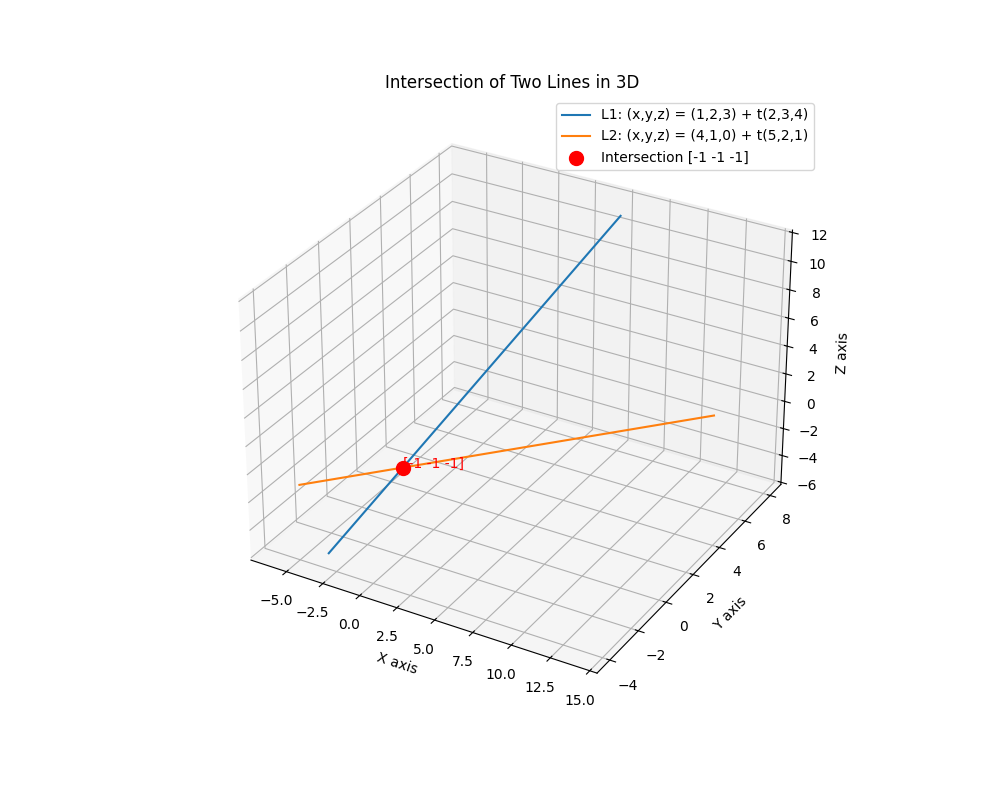
\includegraphics[width=0.75\linewidth]{figs/Figure_1.png}
        \caption{}
        \label{fig:placeholder}
    \end{figure}
\end{frame}
\end{document}
z-euclide}
\usepackage{listings}
\usepackage{adjustbox}
\usepackage{array}
\usepackage{tabularx}
\usepackage{gvv}
\usepackage{lmodern}
\usepackage{circuitikz}
\usepackage{tikz}
\usepackage{graphicx}

\setbeamertemplate{page number in head/foot}[totalframenumber]

\usepackage{tcolorbox}
\tcbuselibrary{minted,breakable,xparse,skins}



\definecolor{bg}{gray}{0.95}
\DeclareTCBListing{mintedbox}{O{}m!O{}}{%
  breakable=true,
  listing engine=minted,
  listing only,
  minted language=#2,
  minted style=default,
  minted options={%
    linenos,
    gobble=0,
    breaklines=true,
    breakafter=,,
    fontsize=\small,
    numbersep=8pt,
    #1},
  boxsep=0pt,
  left skip=0pt,
  right skip=0pt,
  left=25pt,
  right=0pt,
  top=3pt,
  bottom=3pt,
  arc=5pt,
  leftrule=0pt,
  rightrule=0pt,
  bottomrule=2pt,
  toprule=2pt,
  colback=bg,
  colframe=orange!70,
  enhanced,
  overlay={%
    \begin{tcbclipinterior}
    \fill[orange!20!white] (frame.south west) rectangle ([xshift=20pt]frame.north west);
    \end{tcbclipinterior}},
  #3,
}
\lstset{
    language=C,
    basicstyle=\ttfamily\small,
    keywordstyle=\color{blue},
    stringstyle=\color{orange},
    commentstyle=\color{green!60!black},
    numbers=left,
    numberstyle=\tiny\color{gray},
    breaklines=true,
    showstringspaces=false,
}

%\numberwithin{equation}{section}

\title{Matgeo-q.4.4.32}
\author{AI25BTECH11036-SNEHAMRUDULA}

\date{\today} 
\begin{document}

\begin{frame}
\titlepage
\end{frame}

\section*{Outline}
\begin{frame}{question}
    Show that the vectors 
$\myvec{1\\-2\\3}$,\;
$\myvec{2\\3\\-4}$ and 
$\myvec{1\\-3\\5}$ are coplanar.

\end{frame}
\begin{frame}{solution}
\[
\left(\vec{n}^{\,T}\right)\vec{x} = 1
\]
\[
\begin{bmatrix}
1 & -2 & 3 \\
2 & 3 & -4 \\
1 & -3 & 5
\end{bmatrix}
\begin{bmatrix}
l \\ m \\ n
\end{bmatrix}
=
\begin{bmatrix}
1 \\ 1 \\ 1
\end{bmatrix}
\]
The augmented matrix is
\[
\left[
\begin{array}{ccc|c}
1 & -2 & 3 & 1 \\
2 & 3 & -4 & 1 \\
1 & -3 & 5 & 1
\end{array}
\right].
\]
Performing row operations:
\[
R_2 \to R_2 - 2R_1,\quad 
R_3 \to R_3 - R_1
\]
\end{frame}
\begin{frame}{solution}
\[
\left[
\begin{array}{ccc|c}
1 & -2 & 3 & 1 \\
0 & 7 & -10 & -1 \\
0 & -1 & 2 & 0
\end{array}
\right]
\]

Swap \(R_2 \leftrightarrow R_3\):

\[
\left[
\begin{array}{ccc|c}
1 & -2 & 3 & 1 \\
0 & -1 & 2 & 0 \\
0 & 7 & -10 & -1
\end{array}
\right]
\]

Now,
\[
R_3 \to R_3 + 7R_2
\]
\end{frame}
\begin{frame}{solutiionn}
\[
\left[
\begin{array}{ccc|c}
1 & -2 & 3 & 1 \\
0 & -1 & 2 & 0 \\
0 & 0 & 4 & -1
\end{array}
\right]
\]

---

The coefficient matrix is
\[
\begin{bmatrix}
1 & -2 & 3 \\
0 & -1 & 2 \\
0 & 0 & 4
\end{bmatrix}, 
\quad \operatorname{rank} = 3.
\]

The augmented matrix is
\[
\begin{bmatrix}
1 & -2 & 3 & 1 \\
0 & -1 & 2 & 0 \\
0 & 0 & 4 & -1
\end{bmatrix}, 
\quad \operatorname{rank} = 3.
\]
\end{frame}
\begin{frame}{solution}
Since
\[
\operatorname{rank}(\text{Coefficient}) 
= \operatorname{rank}(\text{Augmented}) = 3,
\]
and the number of unknowns is also \(3\), the system has a \textbf{unique solution}.  

\[
\therefore \quad \text{There exists a unique vector } n 
\text{ such that } n^T x = 1 \text{ is the required plane.}
\]
\end{frame}
    \begin{frame}{Graphical Representation}
   \begin{figure}[h!]
\centering
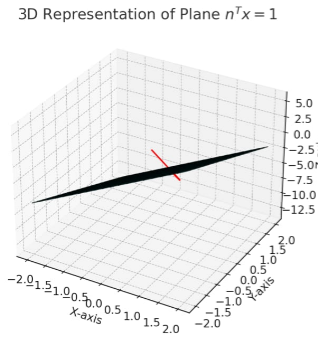
\includegraphics[width=0.6\linewidth]{fig4.4.32.png}
\end{figure}
\end{frame}
\end{document}

